%%% mode: latex
%%% TeX-master: t
%%% End:

\chapter{绪论}
\section{研究背景与意义}
预测问题是经济生活、工业生产、公共卫生和能源系统等众多应用领域的重要问题。若能基于观测的现实预测出未来将要发生的现象,则能为控制或决策提供参考。自然,科学准确的预测是正确决策的重要依据。
然而,现实数据往往是复杂且动态的,难以通过某一确定性的物理定律或因果关系精确推算出未来的状态。因此需要考虑依赖于时间的现象,基于数据自身的历史观测值,建立预测模型从而估计和推测出未来状态,这样处理预测问题的方式被称为时间序列预测。其中,根据数据发生的历史时间顺序所得到的序列观测值即是时间序列数据。
在现实背景下,时间序列数据常常呈现出规模庞大、模态多样和关联复杂等性质,表现出感知度量难、特征融合难和模式挖掘难等问题。
对于这种动态机制不确定的数据,如何建立一种建模技术来解决大规模时间序列数据非平稳状态下的动态性预测问题,对学界和业界都具有重要的理论价值和实际意义。

% \section{研究意义}
在预测科学的发展进程中,各种预测技术和方法推陈出新。
其中,以卷积神经网络(Convolutional neural network,CNN)和循环神经网络(Recurrent neural network,RNN)为代表的深度学习(Deep learning,DL)预测建模技术成为该领域近年来的研究热点。深度学习是一种大数据背景下基于深度神经网络(Deep neural network,DNN)的机器学习(Machine learning,ML)建模思想,着重研究样本数据的内在规律与表示层次~\cite{hintonReducing2006}。相较于传统的统计机器学习方法,即基于统计模型依赖经验选取特征的浅层学习方法,如支持向量机(Support vector machine,SVM)和多层感知机(Multilayer perceptron,MLP)等,DNN采用卷积池化或循环记忆的网络结构,在成功解决了复杂网络结构下训练初始化~\cite{heDelving2015,glorotUnderstanding2010}与梯度不稳定问题~\cite{mikolovContext2012,pascanuDifficulty2013}后,构造的模型具有优异的特征学习能力和预测性能,并根据网络结构的不同,在面对海量时间序列数据时表现出不同的效率与性能侧重优势。

例如,基于卷积结构的DNN(即CNN)预测模型通过卷积与池化,在降低网络参数的同时进行局部特征的抽象表征,使得模型具备良好的学习能力与效率优势;而基于循环结构的DNN(即RNN)预测模型考虑输入数据的时序关系,通过历史的隐藏特征表示与当前的输入数据特征,迭代完成样本的时序特征抽象学习,使得模型具备优异的预测性能。因此,近年来涌现出大量基于深度学习建模技术的预测应用研究,这些技术方法在多项应用领域,如金融市场~\cite{wuImproved2019,zhaoDeep2017,sezerFinancial2020},能源市场~\cite{caiDayahead2019,lindbergLongterm2019,shiDeep2018}和交通管理~\cite{laptevTimeseries2017,wangTraffic2016,xiaoShortterm2019}等,取得了显著的预测效果,表现出良好的应用前景。

尽管深度学习预测建模技术在管理领域中得到不断推广与应用,但研究表明,深度学习模型与浅层学习模型一样受到多种技术因素的影响(如神经网络结构,输入选择和输出策略等)~\cite{sezerFinancial2020,lindbergLongterm2019}。在现实的时间序列预测任务中,这些在其他领域(如图像识别、目标检测、文本分类和机器翻译等)展现出优异性能的深度学习算法会因不恰当的模型参数设置而无法表现出预期性能。此外,深度学习模型普遍依赖梯度下降(Gradient decent,GD)方法~\cite{sutskeverImportance2013,kingmaAdam2015,reddiConvergence2018,allen-zhuConvergence2019,loshchilovDecoupled2019}多次迭代训练其权重参数以优化其预测性能。同时,现有的深度学习预测建模技术普遍依赖人工经验来解决模型神经网络结构设计、参数设置和特征选择等模型选择问题,使得研究人员与从业人员不得不付出高昂的计算开销来摸索与尝试合适的模型参数与输入特征,降低了深度学习建模技术在时间序列预测问题中的应用效率与实际性能。因此,高效解决深度学习预测建模技术中的模型选择问题,以探索和提高其在现实典型时间序列情景中的预测性能和学习效率,是发展时间序列深度学习预测模型及其应用研究中的重要内容。

与梯度下降方法的迭代学习机制不同,随机映射是一种采用非迭代学习机制的神经网络建模方法~\cite{scardapaneRandomness2017,liInsights2017,wang2015jiyu,shen2018jiyu}。随机映射方法通过随机初始化并固定神经网络输入层权重与隐藏层权重,结合闭式求解算法确定输出层权重,构造出随机(Stochastic)神经网络模型。与梯度下降方法构造的训练(Trained)神经网络模型相比,随机神经网络模型具有极低的计算开销、优异的学习效率与良好的非线性表达能力。基于随机映射方法,已发展出极限学习机(Extreme learning machine,ELM)~\cite{shen2017jiyu}、随机向量函数链接网络(Random vector version of the functional-link,RVFL)~\cite{fu2021jiyu}等神经网络学习技术,并在时间序列预测任务中得到了广泛应用~\cite{scardapaneRandomness2017,caoReview2018,tanakaRecent2019}。

然而,基于随机映射的深度神经网络,即随机深度神经网络(Stochastic deep neural network,SDNN),其预测建模技术研究却较未深入。一方面,既有方法多聚焦于随机映射方法的直接应用~\cite{yuImpact2019,huForecasting2020,sunReview2020,hu2021jiyu}或是对现有SDNN模型的组合集成~\cite{wang2018effective,lv2018stacked,lv2019jiyu};另一方面,随机映射方法在大幅提升建模效率的同时,使得所构造的SDNN模型的预测性能对网络结构与参数设置更加敏感,且由于与梯度下降方法在神经网络模型权重参数确定机制上的本质差异,使得传统神经网络建模技术下的模型选择方法对于SDNN预测模型而言适用有限。

此外,SDNN预测模型的模型选择对象及问题,在以卷积和循环为代表的不同特定神经网络结构实现方法下,呈现出个性且复杂的特点。
例如,基于卷积结构的SDNN预测模型在进行模型选择时,区别于传统的训练CNN模型,在卷积结构SDNN模型由多个卷积核组成的随机卷积层中,每个随机卷积核的结构及权重分布都可以是不同的~\cite{zhangErrorfeedback2021};再如,基于循环结构的SDNN预测模型在进行学习建模时,每个循环节点都可生成当前输入的对应目标输出值,区别于传统的训练RNN模型,随机映射方法下其输出权重的闭式求解需考量这些节点的选取与否。
这些特性问题使得基于SDNN的预测建模技术需要考虑不同神经网络结构实现下的方式特点,建立针对且有效的模型选择方法,以更好提升SDNN模型预测效能。

同时,SDNN建模技术在不同结构实现下的特定优化问题外,亦存在区别于传统机器学习方法与随机浅层神经网络模型的共性优化问题。例如,卷积层的单卷积核多通道输入能力\cite{wangTraffic2016}和循环层的单循环节点多时步输入能力\cite{bandaraForecasting2020}均可将单变量时间序列预测建模中的传统一维输入结构提升为二维输入结构,使得时间序列数据在SDNN预测模型中的特征选择这一关键问题更为复杂。


通过对以上背景的分析可知,有必要进行系统、全面、针对且深入的SDNN预测建模技术研究。基于此,本研究在充分利用DNN拓扑结构优异的特征学习能力和随机映射方法低开销与高效率的建模优势基础上,关注SDNN预测建模技术模型选择的问题与挑战,研究SDNN预测模型构造与优化的创新方法与提升策略。

首先,针对SDNN预测模型在不同典型代表结构下实现下的特定问题,例如SDNN预测模型在基于卷积结构实现时的隐藏结构构造与优化问题以及基于循环结构实现时的输出结构构造与优化问题,分别进行深入且细致地探索,创新提出高效且自适应的随机映射卷积隐藏结构构造方法和循环输出结构优化方法;而后,归纳SDNN预测模型在不同结构实现时的共性优化问题,例如特征选择问题,提出一般结构下的SDNN新型时间序列输入特征选择方法;最后,结合不同深度神经网络结构的特有能力优势,例如卷积结构的局部特征学习能力和循环结构的长期特征学习能力,以及考虑SDNN预测建模的整体优化问题,提出混合结构的SDNN预测模型生长与优化方法,构造出强健、鲁棒且准确的SDNN预测建模技术框架。

本研究旨在建立基于随机映射的深度学习预测建模方法,通过结合随机映射方法的建模效率优势与DNN模型的预测性能优势,聚焦既有SDNN预测模型方法的关键问题与挑战,创新提出一系列SDNN预测模型构造与优化方法,并用于解决管理应用中多种复杂现实时间序列预测问题,以期为决策提供更为高效且智能的支持。

在理论层面,本论文将深入研究不同神经网络结构下的SDNN预测模型和新的理论分析框架,如构建基于卷积结构和混合结构的SDNN预测模型的预测误差收敛性分析框架,直观理解SDNN预测模型的构造与决策逻辑。这些新颖的模型与理论分析框架的提出有助于丰富既有SDNN预测建模技术研究的理论体系,具有一定的理论意义。
% ,为完善DNN预测模型的解释性研究提供一定支撑。

在方法层面,本论文将构造多套预测模型构造与优化方法,包括适用于卷积结构、循环结构、一般结构至混合结构SDNN模型的优化技术,形成从特定到一般再到混合的综合技术体系与框架,为SDNN预测建模技术的复杂模型选择问题提供新颖的方法与思路。这些新方法的提出将拓展既有SDNN预测建模技术研究的方法体系,为完善SDNN预测模型的模型选择问题研究提供一定支撑。

在现实层面,本论文将立足于现实时间序列预测任务的多个场景,包括公共卫生领域中的流感阳性样本率预测任务、能源市场中的原油价格预测任务、金融市场中的股票指数预测任务、大气污染中的PM2.5预测任务、电力系统中的电力负荷与电力价格预测任务等。基于模型在不同场景下的预测结果和优势特点,如基于卷积结构SDNN模型的效率优势和基于混合结构SDNN模型的性能优势,可为管理部门制定决策提供效能层面的不同支撑,对SDNN预测建模技术的应用具有良好的现实意义。

\section{研究面临的关键问题}

针对时间序列预测建模这一重要问题,基于SDNN的预测建模技术因其高效的构造效率和良好的预测潜能受到了广泛关注和应用,但既有方法面临着如下关键问题:

(1)如何构建基于卷积结构SDNN预测模型的新颖构造及自适应优化方法,以解决已有卷积结构SDNN预测建模技术中参数选择时的人工依赖、输出权重求解时的病态矩阵和预测过程的不稳定性,是本研究的关键问题。

SDNN模型预测性能对于隐藏结构的设计与参数设置以及输出权重的闭式求解方式非常敏感,这一现象在卷积结构的实现中尤为明显。原因在于,SDNN建模方法下接隐藏层的输入权重与隐藏权重是随机且固定的,输出层权重是基于隐藏特征表征和预测目标的映射通过闭式求解予以确定。更具体的,一方面在卷积结构的SDNN模型实现中,输入层与隐藏层权重统一地被卷积层权重所取代,同时卷积核权重的随机设置与其结构参数息息相关,使得卷积结构SDNN预测模型性能敏感于卷积层结构参数及随机权重,然而既有SDNN的卷积实现方法在进行隐藏卷积结构构造时依赖于人工试错,缺少自适应确定隐藏结构及参数设置的构造与选择方法;另一方面,同时,随着卷积核数量的增加会导致输出层读取的隐藏特征维度呈倍数增大,使得既有的输出层权重求解方法出现病态矩阵问题(Ill-posed problem),从而降低了输出层权重的求解质量,严重影响了模型的拟合能力和预测稳定性。因此,有必要设计一种能够自适应确定隐藏卷积结构及参数,兼具良好预测性能和高效建模效率的SDNN卷积结构实现方法,以更好发挥卷积结构的建模效率优势。

% 通常而言,SDNN模型对时间序列数据的表征通过隐藏层结构的随机映射和输出层的特征学习共同完成。随机映射方法下链接隐藏层的输入权重与隐藏权重是随机且固定的,输出层权重是基于隐藏特征表征和预测目标的映射通过闭式求解予以确定,因此。既有SDNN的卷积实现方法在进行隐藏卷积结构构造时依赖于人工试错,缺少自适应确定隐藏结构及参数设置的构造与选择方法;同时,随着卷积核数量的增加会导致输出层读取的隐藏特征维度呈倍数增大,使得既有的输出层权重求解方法出现病态矩阵问题,从而降低了输出层权重的求解质量,严重影响了模型的拟合能力和预测稳定性。因此,有必要设计一种能够自适应确定隐藏卷积结构及参数,兼具良好预测性能和高效建模效率的SDNN卷积结构实现方法,以更好发挥卷积结构的建模效率优势。

(2)如何构建基于循环结构SDNN预测模型的新颖构造及自适应优化方法,以解决已有循环结构SDNN预测建模技术所忽视的循环隐藏特征表示与预测目标的复杂对应问题,是本研究的关键问题。

区别于直接对局部特征进行高效前馈表征的卷积结构,SDNN循环结构实现方法则更侧重于捕捉与学习时序性特征,利用循环构造当前时间序列观测值与目标值间的映射完成预测建模。在此过程中,每个循环节点都将生成当前读取输入值的对应隐藏特征表示,建立出隐藏特征表示与拟合目标的时间序列对应队列,基于队列内的隐藏特征表示与拟合目标的对应关系闭式求解输出权重。然而,由于时间序列数据的复杂性,队列内的匹配关系并不一定都有助于得到良好的输出权重解。在进行匹配选取时,既有方法采用直接丢弃初始区间的做法,忽视了时间序列隐藏特征表示与拟合目标匹配队列的复杂性,从而降低了输出层权重的求解质量,限制了SDNN循环结构实现方法的时序特征学习能力。因此,有必要设计一种能够自适应确定循环输出结构及参数,兼具良好预测性能和高效建模效率的SDNN循环结构实现方法,以更好发挥循环结构的预测性能潜力。

(3)如何将特征选择与深度神经网络结构相结合,以利用已有SDNN预测模型特征选择方法所忽视的时步多维度输入能力,提出适用于以卷积和循环结构为代表的一般结构SDNN预测模型的自适应特征选择方法,是本研究的关键问题。

与传统机器学习方法或浅层神经网络方法不同,以卷积结构和循环结构为代表的DNN因其隐藏结构的特殊性,如卷积层中的单卷积核多通道结构和循环层中的单循环节点多神经元输入结构,使得DNN预测模型能够将传统的单变量输入的一维特征结构表示在每个输入时步节点囊括入邻近的时域特征,从而将传统一维输入特征作为特例,呈现出复杂的二维输入特征结构表示。此外,相较梯度下降方法训练的DNN预测模型,随机映射方法内在随机机制在提升建模效率的同时,一定程度上降低了模型直接对时间序列原始输入特征进行抽象学习的能力,因此更需要从复杂的输入中挖掘与选择出合适的特征以提升模型预测性能。然而,既有的SDNN预测模型特征选择方法未考虑时间序列输入数据的二维结构性质,仍在一维输入结构表示上进行特征取舍,削弱了特征选择对于SDNN预测模型性能的提升能力。因此,有必要设计一种种能够自适应确定输入特征结构及取舍的SDNN预测模型特征选择方法,以进一步提高模型的预测精度。

(4)如何将不同深度神经网络相结合,以消除已有SDNN预测建模方法固守于某一特定结构的局限,提出可包纳卷积结构、循环结构及其他DNN结构的混合结构SDNN预测模型构造与自适应优化方法,是本研究的关键问题。

面对复杂不同的时间序列预测任务,基于单一结构主体的SDNN预测模型可能难以完全胜任。事实上,SDNN预测模型在不同的神经网络结构实现下侧重不同的特征学习能力,如卷积结构对局部特征的学习能力和循环结构对时序特征的学习能力。故需要混合不同深度神经网络结构,以融合不同结构的性能优势,使SDNN预测模型具备综合的学习能力。然而,既有的SDNN预测建模方法局限于单一结构实现。同时,混合结构的SDNN预测模型对模型参数的选择与建模稳定性提出了更高要求。因此,有必要设计一种可兼容不同种类深度神经网络结构,能够自适应确定隐藏结构组成类别及对应参数,稳健且鲁棒的混合结构SDNN预测模型构造与选择方法,以更好解决时间序列预测问题。

\section{研究内容与创新点}
本文研究目标如下:以精准和高效的时间序列预测为目标,基于随机映射方法与深度神经网络预测模型,构造自适应确定模型参数与特征,准确、高效且稳健的SDNN预测建模技术,以适应复杂不同的时间序列预测场景需要,为管理决策提供更为快捷、智能、安全和稳定的支持。为此,本研究探索SDNN预测建模技术既有方法的关键问题,创新提出对应解决方法和改进策略,利用主流人工时间序列数据和多种现实时间序列数据验证所提方法策略的有效性,以期具备一定的理论意义和良好的现实意义。

\subsection{研究内容}
本研究以高效准确时间序列预测为研究目的,以SDNN预测建模技术为主要研究方法,其主要研究内容如下:

(1)基于卷积结构的SDNN预测模型构造与优化方法

既有SDNN预测模型的卷积结构实现方法依赖于人工设计隐藏结构,其全局更新输出权重的方式易产生不稳定的预测结果,使得随机映射卷积结构的效率优势意义有限。基于此,提出一种基于误差反馈的SDNN预测模型卷积结构构造与优化方法,采用递归添加随机卷积核的方式,逐步构造隐藏结构,通过误差反馈机制局部更新输出权重以此稳步降低模型预测误差,使得所构造模型具有理论保证的收敛误差;同时,利用贪心算法解决卷积结构参数与随机权重选择问题以增强模型感知不同尺度局部特征的能力;最后,结合人工合成时间序列数据、比特币价格、流感阳性样本率、国际原油价格和股票指数时间序列数据,验证所提方法的准确性、收敛性和建模效率。

(2)基于循环结构的SDNN预测模型构造与优化方法

既有SDNN预测模型的循环结构实现方法在采用闭式求解算法计算输出权重时,一般采用直接丢弃循环队列初始区间内隐藏状态与目标间映射关系的方式,这种做法未考虑参与求解的隐藏特征表示与目标队列的复杂关系,限制了随机映射循环结构的预测建模潜能。基于此,考虑堆栈结构、线性解码器结构和循环解码器等不同循环输出结构的实现形式,提出一种基于状态遮掩的SDNN预测模型循环结构构造与优化方法,利用粒子群优化算法对隐藏特征表示与目标队列进行选择以增强模型感知复杂时序特征的能力。同时,结合人工合成时间序列数据、电力负荷和室外温度时间序列数据,从预测准确度和结果稳定性等方面验证所提方法的有效性。

(3)SDNN预测模型的二重特征结构选择方法

既有SDNN预测模型特征选择方法局限于一维的时步单输入结构,其直接对各时步输入特征进行选择的方式未考虑深度神经网络结构对输入时间序列数据的时步多维度结构表示能力,限制了SDNN预测模型的特征学习能力。基于此,提出一种基于输入特征结构变换的二重特征结构优化方法,对输入时间序列的输入步长、时步维度和输入时步加以优化,利用树状帕尔森估计算法优化“时步维度-时步掩码”的输入特征结构元组,完成模型的特征结构选择,进一步提升SDNN模型的时间序列数据学习能力与预测精度。同时,结合人工合成时间序列数据、电力负荷和电力价格时间序列数据,以及不同深度神经网络结构验证所提方法的有效性。

(4)SDNN预测模型的混合结构生长与优化方法

既有SDNN预测模型的构造与选择方法局限于单一的深度神经网络结构,而不同类别的神经网络结构侧重不同的时间序列特征学习能力,现有方法难以主动适应复杂不同的时间序列预测场景。基于此,提出一种基于混合结构的SDNN预测模型生长与优化方法,通过迭代添加不同种类随机深度子网络构造隐藏结构,引入正则项改进误差反馈生长策略以此确定子网络输出权重,建立预优化、子训练和调正则的三阶段优化策略对子网络参数及权重进行优化,以此提升模型的学习能力、预测精度和稳定性。同时,结合人工合成时间序列数据、空气污染和电力负荷时间序列数据,验证所提方法的有效性、必要性、稳定性和收敛性。


\subsection{研究创新点}
基于对面向时间序列预测问题的SDNN预测建模技术理论与应用研究,本文主要创新点如下:

1)针对卷积结构SDNN预测模型中卷积层参数选择及输出权重病态矩阵难题,通过构造误差反馈随机建模构造策略和建立贪心搜索选择方法,提出基于卷积结构的SDNN预测模型构造与优化方法。其创新之处包括以下方面:

(1)通过代数推导证明了基于该方法所构造的预测模型具有随着卷积核的增加而单调下降的预测误差,以此保证了所提方法的收敛性,且其确定的输出权重与既有方法相比具有更小的$L_2$范数,以此提升了模型的预测稳定性;

(2)区别于既有方法仅能用相同宽度的卷积核构造单卷积层,通过贪心选择由不同卷积核宽度组成的备选集,使得模型能够在迭代构造模型的过程中自适应确定卷积参数,其构造的单卷积层具备不同宽度的卷积核,使模型借助单卷积层具备不同尺度局部特征的学习能力;

(3)在人工合成数据、流感阳率数据、国际原油价格数据和股票指数数据上的实验表明,与梯度下降训练的深度神经网络预测模型相比,基于本方法所构造的模型在具备相近甚至更优的预测准确度同时具备极高的建模效率,验证了所提方法的有效性。


2)针对循环结构SDNN预测模型中循环隐藏特征表示与预测目标间的复杂关系处理难题,通过考虑多种SDNN循环输出结构实现方法和利用粒子群优化算法,提出基于循环结构的SDNN预测模型构造与优化方法。其创新之处包括以下方面:

(1)在既有随机映射循环输出结构实现方法外,借鉴梯度下降训练循环神经网络输出结构提出多种随机映射循环输出结构实现方法,并实验分析不同输出结构间的异同优劣,为随机映射循环输出结构的实现应用提供更多支撑;

(2)区别于既有现方法强制丢弃一定初始区间内所有的隐藏状态表示,通过对循环结构每个循环节点生成的隐藏状态表示及目标施加状态掩码,借助粒子群优化方法进行循环队列完整区间内的隐藏状态表示取舍,使得模型能够更好学习输入时间序列数据的时序性特征,降低模型输出权重的学习难度,提升模型的预测性能;

(3)在人工合成数据、电力负荷数据和室外温度数据上的实验表明,与已有的SDNN循环输出结构优化方法相比,所提方法具备更好的多步预测准确度和稳定性,验证了所提方法的有效性。


3)针对以卷积和循环结构为代表的一般SDNN预测模型多输入时步多时步维度特征选择难题,通过构造二维输入特征结构和利用树状帕尔森估计算法,提出了SDNN预测模型的二重特征结构选择方法。其创新之处包括以下方面:

(1)区别于既有SDNN特征选择方法局限于一维输入结构,且仅利用时步掩码对输入特征进行选择的方式,基于以卷积结构和循环结构为代表的深度神经网络时步多维度特征读取能力,利用滑动窗口构造出时步多维度的新颖输入特征结构,丰富模型输入信息;

(2)将既有的多输入特征选择方法作为被囊括的特例,通过树状帕尔森估计算法对输入的二维特征结构时步维度和时步掩码参数同时进行优化,使得模型能够根据不同的时间序列任务在每个时步输入节点丰富邻近特征信息的同时,去除冗余和嘈杂的输入时步节点,降低模型抽象特征的学习难度,提升模型的预测性能;

(3)在人工合成数据、电力负荷数据和电力价格数据上的实验表明,与已有的SDNN特征选择方法相比,基于所提方法构造的模型具有更优的预测性能,验证了所提方法的有效性。

4)针对混合卷积、循环和其他深度神经网络结构的SDNN预测模型构造与自适应优化难题,通过改进误差反馈生长策略和建立三阶段优化算法,提出了SDNN预测模型的混合结构生长与优化方法。其创新之处包括以下方面:

(1)区别于既有SDNN预测模型传统的单一隐藏神经网络结构,构造混合结构的生长策略,通过矩阵分析证明了基于该策略所构造的预测模型随着不同结构子网络的加入具有单调下降的预测误差,以此保证了所提方法的收敛性,且通过向输出权重的计算过程引入正则项,避免了既有随机映射方法更新输出权重时可能遇到的病态矩阵问题和过拟合问题,提升了模型的鲁棒性;

(2)区别于既有SDNN参数优化方法仅对部分参数进行选择的做法,提出预优化、子训练和调正则的三阶段优化方法对定义子网络的结构参数、输入与隐藏权重参数,以及输出权重进行完整优化,使得模型能够根据不同的时间序列任务自适应地生长神经网络结构与选择参数,进一步提升模型预测性能;

(3)在人工合成数据、空气污染数据和电力负荷数据上的实验表明,与已有的先进SDNN预测模型相比,基于所提方法构造的模型具有更优的预测性能,验证了所提方法的有效性。

% \clearpage
\begin{figure}[!t]
    \centering
    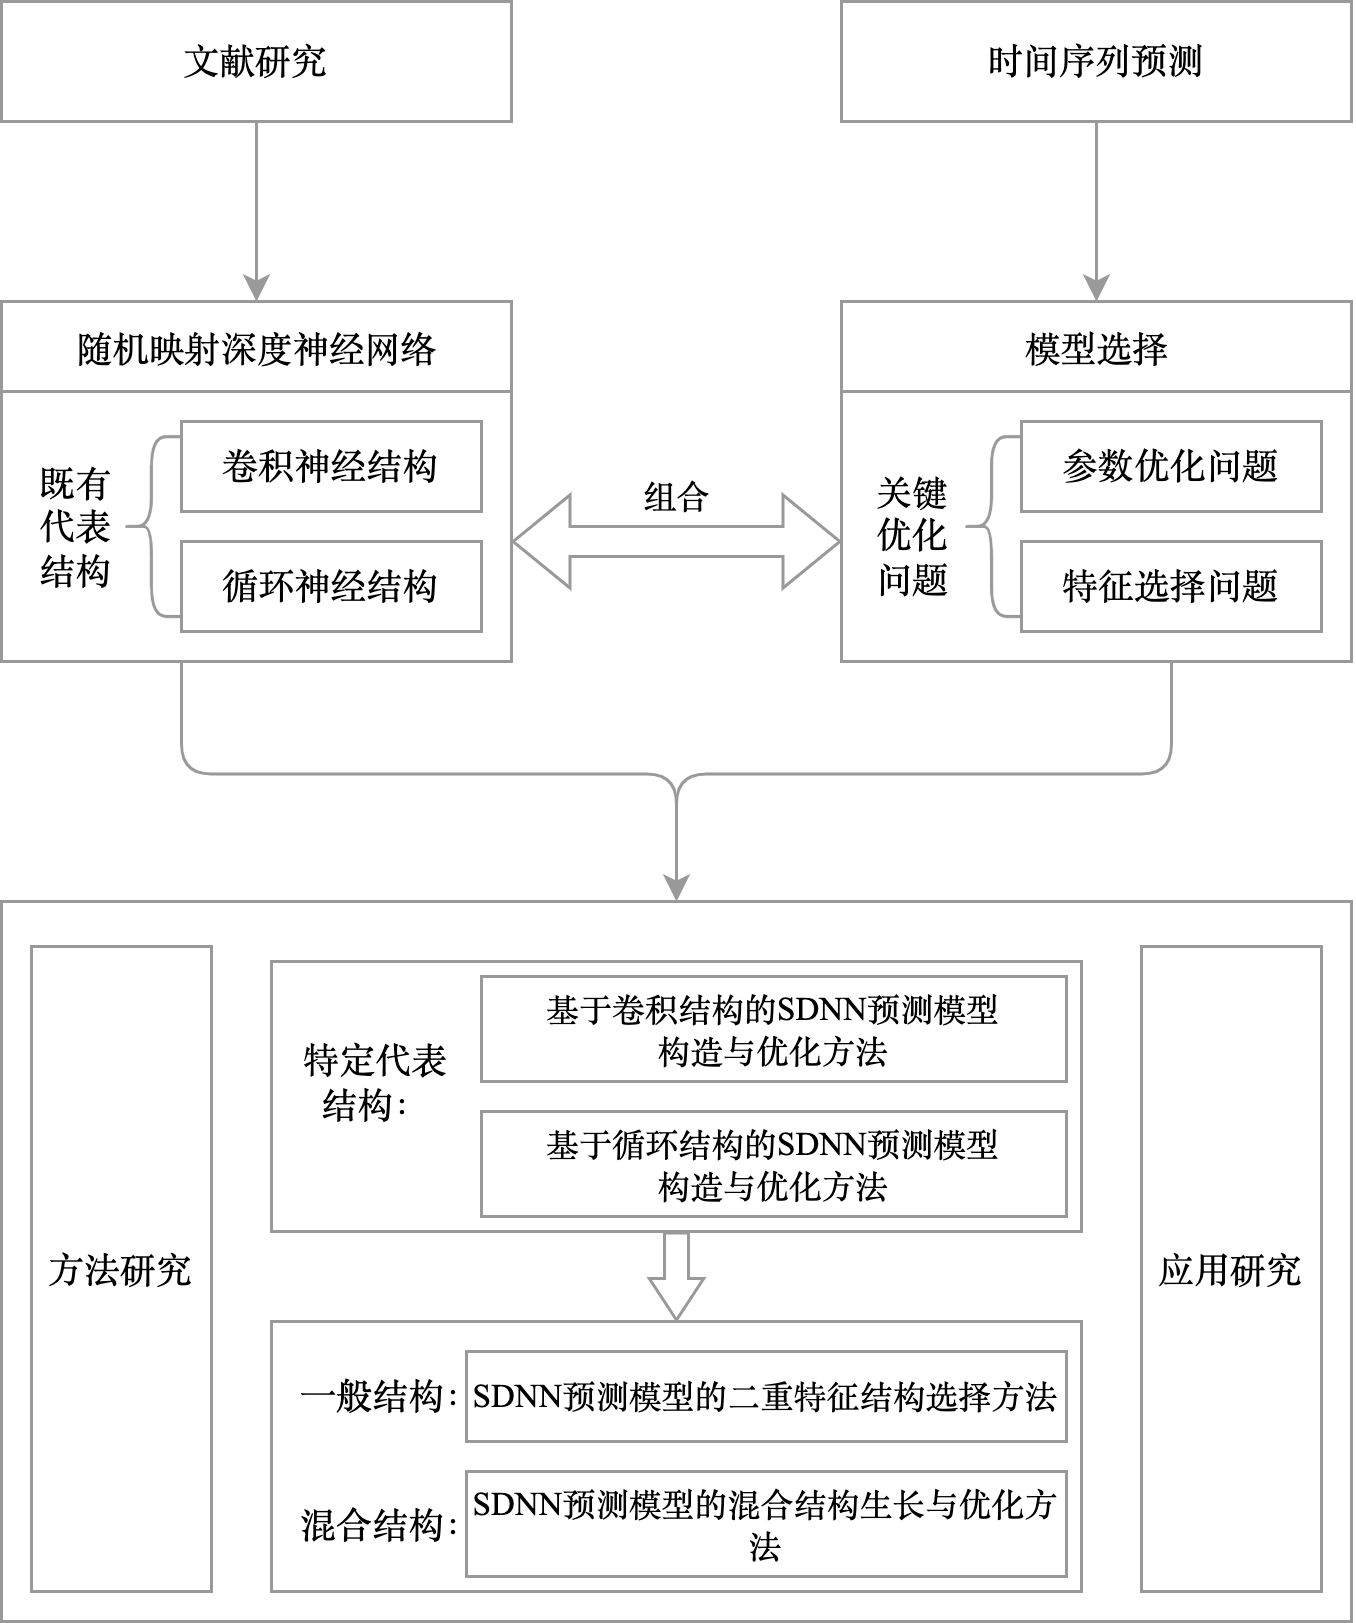
\includegraphics[width=0.8\linewidth]{float/ch.intro/thesis_arch.png}
    \caption{\label{fig:body}本研究技术路线}
\end{figure}
\section{技术路线与论文结构}
\subsection{技术路线\label{sec:thesisRoad}}
本研究以时间序列预测问题为背景,结合随机映射方法的建模效率与深度神经网络的学习潜能,基于SDNN预测建模技术进行方法研究和现实应用。
本研究的技术路线如\autoref{fig:body}所示,通过文献研究法分析SDNN预测建模技术的背景、现状与不足,归纳以卷积神经网络和循环神经网络结构为代表的既有SDNN建模方法,从参数优化与特征选择两方面,系统分析其在时间序列预测建模时的模型选择关键优化问题。

首先,针对不同特定代表结构下的SDNN模型参数优化个性问题展开研究,分别构造基于卷积结构的SDNN预测模型构造与优化方法,以及基于循环结构的SDNN预测模型构造与优化方法;而后,将典型且个性的特定结构研究在神经网络结构层面予以推广,关注以卷积结构与循环结构为代表的一般结构下SDNN预测模型的特征选择问题,提出兼容不同深度神经网络结构的二重特征结构选择方法,并进一步考虑混合不同神经网络结构的SDNN模型参数优化问题,提出SDNN模型的混合结构生长与优化方法。
在此技术路线中,结合主流人工合成时间序列数据与多种复杂的现实时间序列数据,通过准确性比较实验、收敛性验证实验和消融实验,结合定量对比与机器学习理论分析,验证所提方法的有效性。

\begin{figure}[!t]
    \centering
    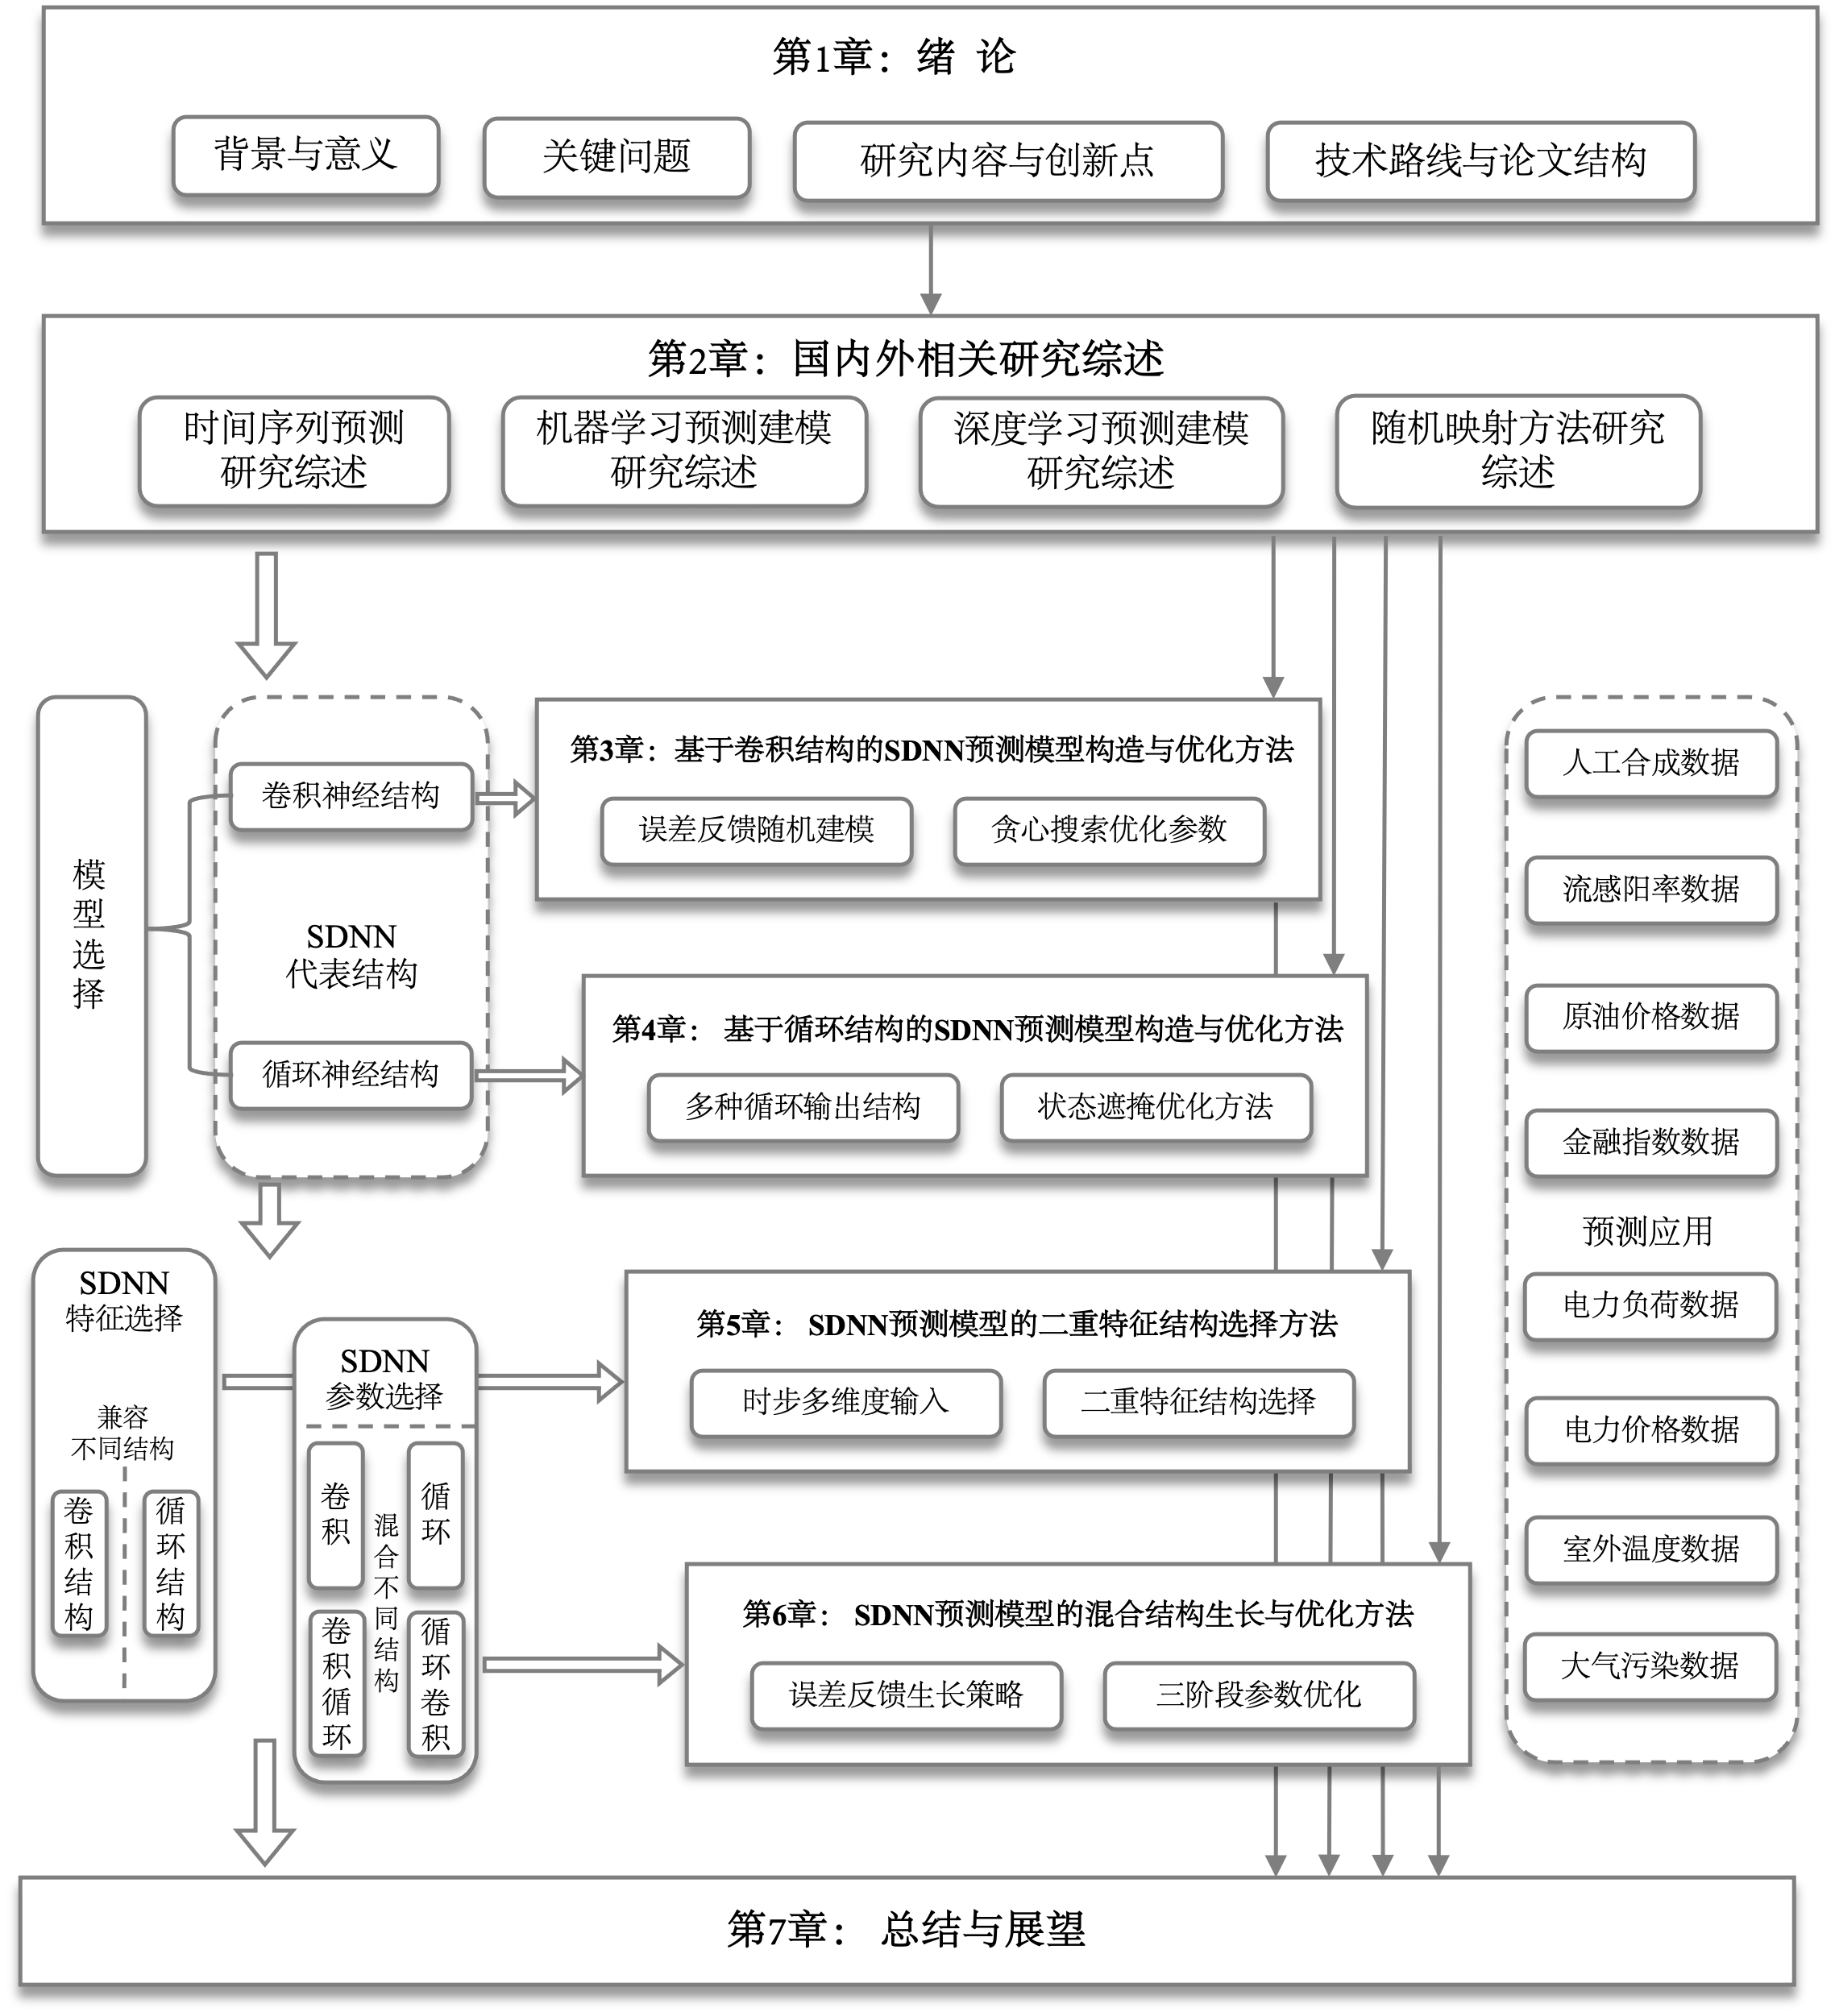
\includegraphics[width=0.95\linewidth]{float/ch.intro/thesis_content.png}
    \caption{\label{fig:body.arch}本论文主要结构}
\end{figure}

% \clearpage
\subsection{论文结构}
全文共七章,主要结构如\cref{fig:body.arch}所示,各章内容如下:

第1章~绪论:介绍了本研究的背景与意义、所面临的关键问题、主要的研究内容与创新点、研究内容间的技术路线及全文结构。

第2章~国内外相关研究综述:介绍了时间序列预测问题的定义、机器学习预测建模技术至深度学习预测建模技术的演进与现状、随机映射方法的动机及随机映射深度学习预测建模技术的现状及不足。

第3章~基于卷积结构的SDNN预测模型构造与优化方法:提出误差反馈随机建模构造方法及贪心搜索参数优化方法,建立出一种高效且收敛的卷积结构SDNN预测模型,结合人工合成数据、流感阳率数据、原油价格数据和金融指数数据的预测问题进行实验验证。

第4章~基于循环结构的SDNN预测模型构造与优化方法:考量多种随机映射循环输出结构及提出基于粒子群优化的状态遮掩优化方法,建立出一种改进的循环结构SDNN预测模型,结合人工合成数据、电力负荷数据和室外温度数据的预测问题进行实验验证。

第5章~SDNN预测模型的二重特征结构选择方法:构造兼容卷积结构与循环结构深度神经网络的时间序列数据二维输入特征结构及提出基于树状帕尔森估计的二重特征结构选择方法,建立出基于改进特征选择的SDNN预测模型,结合人工合成数据、电力负荷数据和电力价格数据的预测问题进行实验验证。

第6章~SDNN预测模型的混合结构生长与优化方法:改进误差反馈生长策略及提出子网络参数的三阶段优化方法,建立出一种准确、收敛且稳健的混合结构SDNN预测模型,结合人工合成数据、空气污染数据和电力负荷数据的预测问题进行实验验证。

第7章~总结与展望:总结本研究的主要内容、不足之处及改进方向。

其中,第3章至第6章为本文的主要研究内容章节,其逻辑关系在于以下方面:

(1)第3章与第4章为并列关系,该两章主要研究内容是第5章与第6章研究内容的基础。具体地,本研究聚焦基于随机映射的时间序列深度学习预测建模技术,卷积结构和循环结构作为既有深度神经网络的代表结构,本文第3章与第4章分别针对深度神经网络基于随机映射方法在特定于卷积结构和循环结构实现下的构造与优化问题展开研究,解决了既有卷积结构实现方法的性能瓶颈,改进了既有循环结构实现方法的输入输出映射,提升了在卷积结构和循环结构这类特定深度神经网络结构实现上的SDNN预测模型准确性。

(2)基于输入特征选择视角,第5章是对第3、4章内容的改进。具体地,凝练第3章与第4章所述SDNN卷积结构和循环结构对时步多维度输入能力的支持共性,设计了兼容卷积结构和循环结构的SDNN预测模型二重特征结构选择方法,突破了既有SDNN预测模型特征选择方法在一维输入结构上的局限,提升了基于卷积结构和循环结构的一般深度神经网络结构下的SDNN预测模型准确性。

(3)基于整体参数优化视角,第6章是对第3、4章内容的改进。具体地,将第3章与第4章所述SDNN卷积结构和循环结构作为超参数控制下的子网络结构状态,提出自适应混合多种不同特定类型子网络的SDNN预测生长策略,建立对子网络在生长过程中超参数、编码过程权重参数和生成过程权重参数的整体参数优化方法,进一步提升了自适应选择卷积结构和循环结构等混合深度神经子网络结构下的SDNN预测模型准确性。



% 第六章 总结与展望:本章对全文的研究工作进行总结,指出本文研究的不足和未来的展望。

% % \section{课题来源}
% % 本课题来源于:

% % 国家自然科学基金面上项目:基于多输出支持向量回归的预测技术研究(立项时间:2016-01,项目编号:71571080)。

% % 国家自然科学基金面上项目:大数据环境下基于计算智能的预测建模技术及其在电力负荷预测中的应用(立项时间:2019-01,项目编号:71871101)。

% % 国家电网公司华中分部科技项目:华中区域共享型电力交易与服务平台关键技术研究(立项时间:2020-03,项目编号:52140019000U)。